\documentclass[english,,man]{apa6}
\usepackage{lmodern}
\usepackage{amssymb,amsmath}
\usepackage{ifxetex,ifluatex}
\usepackage{fixltx2e} % provides \textsubscript
\ifnum 0\ifxetex 1\fi\ifluatex 1\fi=0 % if pdftex
  \usepackage[T1]{fontenc}
  \usepackage[utf8]{inputenc}
\else % if luatex or xelatex
  \ifxetex
    \usepackage{mathspec}
  \else
    \usepackage{fontspec}
  \fi
  \defaultfontfeatures{Ligatures=TeX,Scale=MatchLowercase}
\fi
% use upquote if available, for straight quotes in verbatim environments
\IfFileExists{upquote.sty}{\usepackage{upquote}}{}
% use microtype if available
\IfFileExists{microtype.sty}{%
\usepackage{microtype}
\UseMicrotypeSet[protrusion]{basicmath} % disable protrusion for tt fonts
}{}
\usepackage{hyperref}
\hypersetup{unicode=true,
            pdftitle={Thinking About Patterns Over Time},
            pdfauthor={Christopher R. Dishop, Michael T. Braun, Goran Kuljanin, \& Richard P. DeShon},
            pdfkeywords={longitudinal inferences, between-unit, growth, trends, dynamics,
relationships over time, processes},
            pdfborder={0 0 0},
            breaklinks=true}
\urlstyle{same}  % don't use monospace font for urls
\ifnum 0\ifxetex 1\fi\ifluatex 1\fi=0 % if pdftex
  \usepackage[shorthands=off,main=english]{babel}
\else
  \usepackage{polyglossia}
  \setmainlanguage[]{english}
\fi
\usepackage{graphicx,grffile}
\makeatletter
\def\maxwidth{\ifdim\Gin@nat@width>\linewidth\linewidth\else\Gin@nat@width\fi}
\def\maxheight{\ifdim\Gin@nat@height>\textheight\textheight\else\Gin@nat@height\fi}
\makeatother
% Scale images if necessary, so that they will not overflow the page
% margins by default, and it is still possible to overwrite the defaults
% using explicit options in \includegraphics[width, height, ...]{}
\setkeys{Gin}{width=\maxwidth,height=\maxheight,keepaspectratio}
\IfFileExists{parskip.sty}{%
\usepackage{parskip}
}{% else
\setlength{\parindent}{0pt}
\setlength{\parskip}{6pt plus 2pt minus 1pt}
}
\setlength{\emergencystretch}{3em}  % prevent overfull lines
\providecommand{\tightlist}{%
  \setlength{\itemsep}{0pt}\setlength{\parskip}{0pt}}
\setcounter{secnumdepth}{0}
% Redefines (sub)paragraphs to behave more like sections
\ifx\paragraph\undefined\else
\let\oldparagraph\paragraph
\renewcommand{\paragraph}[1]{\oldparagraph{#1}\mbox{}}
\fi
\ifx\subparagraph\undefined\else
\let\oldsubparagraph\subparagraph
\renewcommand{\subparagraph}[1]{\oldsubparagraph{#1}\mbox{}}
\fi

%%% Use protect on footnotes to avoid problems with footnotes in titles
\let\rmarkdownfootnote\footnote%
\def\footnote{\protect\rmarkdownfootnote}


  \title{Thinking About Patterns Over Time}
    \author{Christopher R. Dishop\textsuperscript{1}, Michael T.
Braun\textsuperscript{2}, Goran Kuljanin\textsuperscript{3}, \& Richard
P. DeShon\textsuperscript{1}}
    \date{}
  
\shorttitle{LONGITUDINAL INFERENCES}
\affiliation{
\vspace{0.5cm}
\textsuperscript{1} Michigan State University\\\textsuperscript{2} University of South Florida\\\textsuperscript{3} DePaul University}
\keywords{longitudinal inferences, between-unit, growth, trends, dynamics, relationships over time, processes}
\usepackage{csquotes}
\usepackage{upgreek}
\captionsetup{font=singlespacing,justification=justified}

\usepackage{longtable}
\usepackage{lscape}
\usepackage{multirow}
\usepackage{tabularx}
\usepackage[flushleft]{threeparttable}
\usepackage{threeparttablex}

\newenvironment{lltable}{\begin{landscape}\begin{center}\begin{ThreePartTable}}{\end{ThreePartTable}\end{center}\end{landscape}}

\makeatletter
\newcommand\LastLTentrywidth{1em}
\newlength\longtablewidth
\setlength{\longtablewidth}{1in}
\newcommand{\getlongtablewidth}{\begingroup \ifcsname LT@\roman{LT@tables}\endcsname \global\longtablewidth=0pt \renewcommand{\LT@entry}[2]{\global\advance\longtablewidth by ##2\relax\gdef\LastLTentrywidth{##2}}\@nameuse{LT@\roman{LT@tables}} \fi \endgroup}


\DeclareDelayedFloatFlavor{ThreePartTable}{table}
\DeclareDelayedFloatFlavor{lltable}{table}
\DeclareDelayedFloatFlavor*{longtable}{table}
\makeatletter
\renewcommand{\efloat@iwrite}[1]{\immediate\expandafter\protected@write\csname efloat@post#1\endcsname{}}
\makeatother
\usepackage{lineno}

\linenumbers

\authornote{\ldots{}.

Correspondence concerning this article should be addressed to
Christopher R. Dishop, 316 Physics Road, Psychology Building, Room 348,
East Lansing, MI, 48823. E-mail:
\href{mailto:dishopch@msu.edu}{\nolinkurl{dishopch@msu.edu}}}

\abstract{
This paper is about how to think about patterns contained in
longitudinal or panel data structures. Organizational scientists
recognize that psychological phenomena and processes unfold over time
and, to better understand them, organizational researchers increasingly
work with longitudinal data and explore inferences within those data
structures. Longitudinal inferences may focus on any number of
fundamental patterns, including construct trajectories, relationships
between constructs, or dynamics. Although the diversity of longitudinal
inferences provides a wide foundation for garnering knowledge in any
given area, it also makes it difficult for researchers to know the set
of inferences they may explore with longitudinal data, which statistical
models to use given their question, and how to locate their specific
study within the broader set of longitudinal inferences. Studies that
collect longitudinal data often only focus on one inference category
when they could be asking about many more fundamental patterns and
learning additional insights about their process of interest. Moreover,
a recent article noted that certain statistical models are inappropriate
for inferences about dynamics, so it is important for researchers to
know how dynamic inferences differ from other, related ways of thinking
about patterns over time such as relationships and trend. In this paper,
we develop a framework to describe the variety of between-unit research
questions and inferences researchers may explore with longitudinal data
-- we demonstrate how to think about these fundamental patterns.


}

\usepackage{amsthm}
\newtheorem{theorem}{Theorem}[section]
\newtheorem{lemma}{Lemma}[section]
\theoremstyle{definition}
\newtheorem{definition}{Definition}[section]
\newtheorem{corollary}{Corollary}[section]
\newtheorem{proposition}{Proposition}[section]
\theoremstyle{definition}
\newtheorem{example}{Example}[section]
\theoremstyle{definition}
\newtheorem{exercise}{Exercise}[section]
\theoremstyle{remark}
\newtheorem*{remark}{Remark}
\newtheorem*{solution}{Solution}
\begin{document}
\maketitle

Organizational scientists recognize that psychological phenomena and
processes unfold over time (Beal, 2015; Pitariu \& Ployhart, 2010).
Individuals in the workplace, over time, strive to accomplish work
goals, team members collaborate so the whole eventually becomes greater
than the sum of its parts, and managers repeatedly promote values to
build vibrant, innovative work cultures. To better understand
psychological phenomena, such as motivation, teamwork, and
organizaitonal culture, researchers must attent not to static snapshots
of behavior (Ilgen \& Hulin, 2000; Kozlowski, Chao, Grand, Braun, \&
Kuljanin, 2013, 2016) but to variables and relationships as they move
through time. Obtaining longitudinal data allows researchers to capture
the unfolding set of events, interactions, behaviors, cognitions, or
affective reactions across a variety of psychological phenomena.

Researchers have the opportunity to explore many inferences when they
analyze longitudinal data. For example, researchers may examine the
shape of trajectories on psychological constructs (e.g., Did job
satisfaction generally increase or decrease during the past six
months?), how two or more constructs relate to each other (e.g., Did
team communication and cohesion positively correlate over time?), or
whether changes in one variable relate to changes in another (e.g., Did
changes in goal-setting relate to changes in employee performance?
Dunford, Shipp, Boss, Angermeier, \& Boss, 2012; Hardy, Day, \& Steele,
2018; Jones et al., 2016; Judge, Simon, Hurst, \& Kelley, 2014; Lanaj,
Johnson, \& Wang, 2016; Rosen, Koopman, Gabriel, \& Johnson, 2016; Scott
\& Barnes, 2011). Given the variety of available inferences with
longitudinal data, an organizing framework would elucidate their subtle
differences and enhance theoretical insight.

We developed a framework that organizes the fundamental between-unit
patterns that researchers may explore with longitudinal data. In this
paper, we use it to describe how to think about patterns contained in
longitudinal or panel data structures. Our manuscript is timely for two
reasons. First, it consolidates disparate literature. The ways of
thinking (i.e., inference categories) that we describe are not new, they
are contained in the organizational literature already, but they are
often discussed in isolation which limits a common understanding of how
they fit together. To demonstrate this point, we conducted a brief
review of articles published in the \emph{Journal of Applied Psychology}
and the \emph{Journal of Business and Psychology} in the years 2017 and
2018 that contained three or more waves of data with every variable
measured at each time point. Twenty-eight studies were identified and,
using the study hypotheses, introductions, and discussions, classified
according to the inference categories that we discuss in this paper.
Table 1 reports the frequencies of each inference across the 28 studies.
The specific inference categories (trend, relationships, and dynamics)
will be fully developed later, what matters here is that a majority of
the reviewed studies explored a single inference category, and no study
focused on all three. We are not saying that empirical research must
focus on a broader set of inferences and questions when they explore
longitudinal data, but we are pointing out that other inferences and
ways of thinking about patterns exist that researchers may not be aware
of. This paper presents each inference in a single location rather than
forcing researchers to locate and parse disparate literature to
understand what they can ask of longitudinal data. Second, a recent
article noted that, despite a growing emphasis on dynamics in
organizational science, certain statistical models are inappropriate for
inferences about dynamics (Xu, DeShon, \& Dishop, in press). The authors
state that researchers should consider whether their interest is on
dynamics or other over time patterns and choose their statistical model
accordingly. Researchers, therefore, need to know how dynamic inferences
differ from other, related inferences. Here, we fully describe those
differences.

\hypertarget{longitudinal-research-in-applied-psychology}{%
\section{Longitudinal Research in Applied
Psychology}\label{longitudinal-research-in-applied-psychology}}

This paper is devoted to inferences with repeated measures, so we begin
with a few labels and definitions. Authors typically identify a
\enquote{longitudinal} study by contrasting either (a) research designs
or (b) data structures. Longitudinal \emph{research} is different from
cross-sectional research because longitudinal designs entail three or
more repeated observations (Ployhart \& Vandenberg, 2010). We therefore
emphasize differences on the number of observations when we distinguish
longitudinal from other types of research. Longitudinal or panel
\emph{data} are repeated observations on several units (i.e., \(N\) or
\(i\) \textgreater{} 1), whereas time-series data are observations of
one unit over time -- a distinction that focuses on the amount of people
in the study (given repeated measures). Most organizational studies
collect data on more than one unit, therefore our discussion below
focuses on longitudinal research with panel data, or designs with \(N\)
\textgreater{} 1, \(t\) \(\geq\) 3, and the same construct(s) measured
on each \(i\) at each \(t\). That is, we focus on designs with repeated
measures across many people (units) where every variable is measured at
each time point.

Longitudinal applies to both short and long-term research. An experiment
with ten trials is longitudinal, as is a study spanning 10 years that
assesses its measures once every year. Longitudinal is not reserved for
\enquote{long-term} studies that last more than one year irrespective of
the frequency of their observations. Rather, certain processes unfold
over short time horizons (e.g., decision-making on simple tasks, swift
action teams; Wildman et al., 2012) whereas other psychological
phenomena unfold over long time horizons (e.g., the development of a
shared organizational culture; Mitchell \& James, 2001), so the
informativeness of a particular study depends on its rationale, research
design, analytical work, and effective interpretation of results -- as
with any study. Short and long time horizons both offer valuable
insights.

\hypertarget{framework-for-longitudinal-inferences}{%
\section{Framework for Longitudinal
Inferences}\label{framework-for-longitudinal-inferences}}

We use three inference categories to partition our discussion, including
trends, relationships, and dynamics. Briefly, longitudinal inferences
focusing on trends assess whether trajectories follow a predictable
pattern or whether trajectories differ between-units; longitudinal
inferences focusing on relationships between constructs assess the
between-unit relationship among one or more constructs; longitudinal
inferences focusing on dynamics in constructs assess how one or more
constructs move through time as functions of themselves and each other
and emphasize how the past constrains the future. Each category comes
with box-and-arrow model heuristics\footnote{Note that statistical
  models differ from the term, \enquote{model heuristic.} A model
  heuristic is a visual representation only, whereas a statistical model
  is characterized by a formula explaining the data and assumptions on
  the errors, and the parameters of statistical models are estimated
  using an estimation technique. In this paper, we never use the term,
  \enquote{model} without pairing it either with \enquote{statistical}
  or \enquote{heuristic} -- the two differ substantially.} that
represent the broad inferences, research questions to orient the reader
as to what the sub-inferences capture (i.e., inferences are the answers
to the research questions that we present), and references for where to
find statistical models that are appropriate for a given inference.

Although we use box-and-arrow diagrams throughout to represent the broad
inferences, we also graph a few of the more challenging inferences with
mock data -- some of the inferences in the trend and relationships
sections are difficult to grasp without seeing them in data form. Keep
in mind, however, that data are always messy. It is rare to find data in
which the inferences present themselves simply by plotting -- althought
it is certainly possible. We use these \enquote{data plots} to clearly
convey what the inferences mean, but be aware that field data are often
noisy.

Finally, despite pointing researchers to statistical models, our paper
puts a majority of its emphasis on inferences, therefore researchers
need to be sure that they appreciate all of the nuance before applying a
recommended statistical model. Numerous issues arise when modeling
longitudinal data and the statistical models differ in how they handle
these issues, the assumptions they make, and the data format they
require. We do not speak directly to those issues here, but we refer
readers to a number of informative references for each statistical
model.

\begin{figure}

{\centering 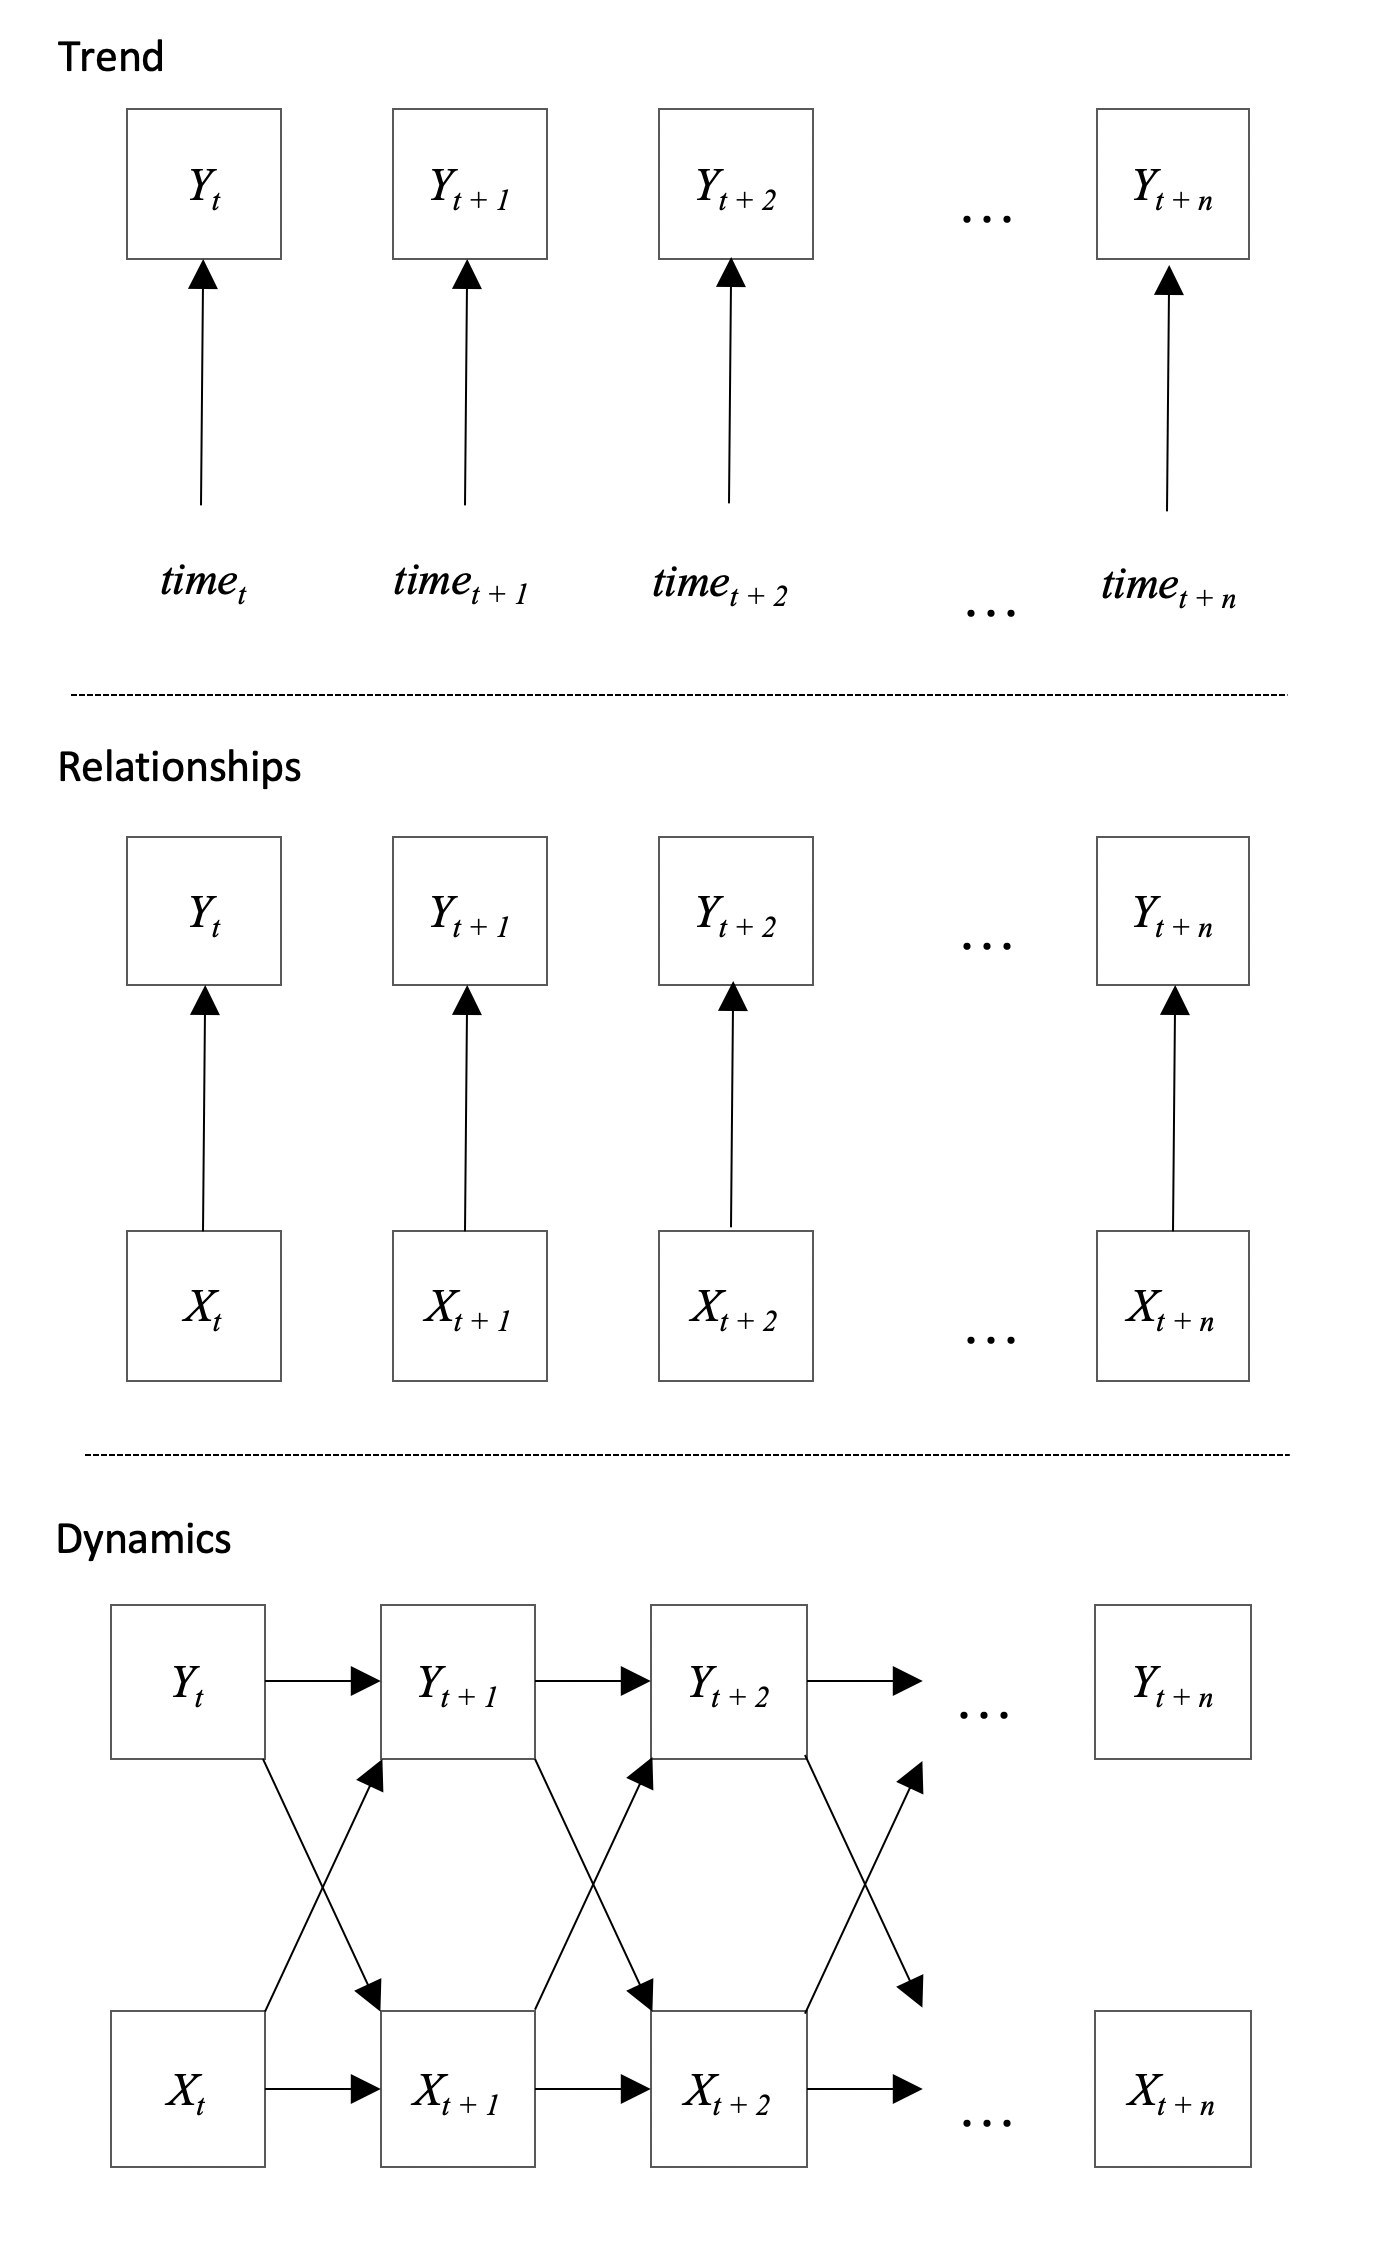
\includegraphics[width=4.66in]{figures/dynamics/framework} 

}

\caption{Common inference categories with models applied to longitudinal data.\label{framework_figure}}\label{fig:unnamed-chunk-6}
\end{figure}

\begin{longtable}[t]{>{\raggedright\arraybackslash}p{15em}>{\raggedright\arraybackslash}p{15em}}
\caption{\label{tab:unnamed-chunk-7}\label{inference_frequencies}Number of times a recent article emphasized one or more inference category.}\\
\toprule
Type & Occurence\\
\midrule
\endfirsthead
\caption[]{\label{tab:unnamed-chunk-7}Number of times a recent article emphasized one or more inference category. \textit{(continued)}}\\
\toprule
Type & Occurence\\
\midrule
\endhead
\
\endfoot
\bottomrule
\endlastfoot
Trend & 4\\
Relationships & 13\\
Dynamics & 10\\
Any 2 & 1\\
All 3 & 0\\*
\end{longtable}

\hypertarget{trend}{%
\section{Trend}\label{trend}}

Made popular in the organizational literature by Bliese and Ployhart
(2002) and Chan (1998), trend inferences represent a class of thinking
in which researchers create an index of time and relate it to their
response variable to understand the trajectory of the dependent
variable. The first panel of Figure \ref{framework_figure} shows a
box-and-arrow model heuristic in which time is related to an outcome,
\(y\), and ultimately the analyst is interested in a variety of
questions about trend and its correlates. Trend inferences have two
components: trend itself and level. For clarity, we discuss them
separately.

\hypertarget{component-1---trend}{%
\subsubsection{Component 1 - Trend}\label{component-1---trend}}

Does affect, in general, increase or decrease across time, or is its
trajectory relatively flat? Does trainee skill generally increase over
the training session? These are questions about trend, and these first
two are specifically about linear trend. It is also possible to explore
how variables bend or curve across time. Do newcomer perceptions of
climate increase and then plateau over time? Does the response time of a
medical team decrease with each successive case but then remain stable
once the team can no longer improve their coordination? These latter
questions concern curvilinear trajectories.

Trend has to do with the systematic direction or global shape of a
trajectory across time. If we put a variable on the \(y\)-axis and plot
its values against time on the \(x\)-axis, do the values display a
stable temporal pattern? It can be thought of as the coarse-grained
direction of a trajectory. A positive trend indicates that, on average
across units, we expect the variable to increase over time and a
negative trend indicates that we expect the variable to decrease over
time. Our first trend research question, therefore, concerns the shape
of the trajectory.

\begin{quote}
\begin{quote}
\textbf{Research Question 1:} On average across units, is there a
positive/negative/curvilinear trend?
\end{quote}
\end{quote}

Many research questions and inferences begin with the average pattern
(or relationship) and then move to variability, the same applies here.
After learning about the average trend across the sample, researchers
then focus on trend variability. How much consistency is there in the
trend pattern? Do all trainees develop greater skill across time? Is
there variability in the trend of helping behaviors, or
counterproductive work behaviors over time?

\begin{quote}
\begin{quote}
\textbf{Research Question 2:} Does trend differ across units?
\end{quote}
\end{quote}

Research questions one and two concern one variable, but they can also
be iterated across all observed variables. For example, we might
discover that -- on average across units -- affect and performance
trends both decrease, but there is greater variability across units in
the affect trend. Or we might learn that affect has a negative trend
while performance has a positive trend.

Correlating these trends between-units is the next inference.
Correlating indicates co-occuring patterns, where a large, positive,
between-unit correlation between affect and performance trends indicates
that people with a positive affect trend (usually) have a positive
performance trend and people with a negative affect trend (usually) have
a negative performance trend.

Figure \ref{trend_correlation} shows the inuition behind this inference
with a set of graphs. In Panel A, we plot affect and performance across
time for three individuals. Affect goes up while performance goes down
for person one, this pattern is reversed for person two, and person
three reports trendless affect and performance (i.e., zero trend). We
use different colors to label the trends for each person. The affect and
performance trends for person one are labeled with red lines, whereas
person two has green lines and person three has blue lines.

Panel B then maps those pairings onto a scatterplot that demonstrates
the between-unit relationship among affect and performance trends. For
example, person one has a positive affect trend and a negative
performance trend, so their value in Panel B goes on the bottom right,
whereas person two has the opposite pattern and therefore is placed on
the top left (where the performance trend is positive and the affect
trend is negative). Producing this bottom scatter plot tells us that the
between-unit association among affect and performance trends is
negative. That is, people with a positive affect trend are expected to
have a negative performance trend, people with a negative affect trend
are expected to have a positive performance trend, and people with an
affect trend of zero are expected to have a performance trend of zero.

\begin{center}

------------

Insert Figure \ref{trend_correlation} about here

------------

\end{center}

\begin{quote}
\begin{quote}
\textbf{Research Question 3:} What is the between-unit correlation among
two trends?
\end{quote}
\end{quote}

The final trend inference is about identifying covariates or predictors
of trend. Does gender predict depletion trends? Does the trend in unit
climate covary with between-unit differences in leader quality?

Figure \ref{trend_covariate} demonstrates the inference in a plot. We
graph affect across time for six employees that differ by job type. The
first three individuals work in research and development, whereas the
final three work in sales. Affect trajectories tend to decrease over
time for employees in research and development, whereas affect
trajectories tend to increase for those in sales. An individual's job
type, then, gives us a clue to their likely affect trend -- said
formally, job type covaries with affect trend, such that we expect
individuals in sales to have positive affect trends and individuals in
research and development to have negative affect trends. The expected
trends are plotted as the thick blue lines.

\begin{center}

------------

Insert Figure \ref{trend_covariate} about here

------------

\end{center}

\begin{quote}
\begin{quote}
\textbf{Research Question 4:} What is the betweeen-unit correlation
among trend and a covariate?
\end{quote}
\end{quote}

Note the difference between research questions three and four. Both are
between unit, but three is about co-occuring trend patterns whereas four
is about the relationship between trend and a covariate/predictor. With
respect to our examples, inference three (i.e., the answer to research
question three) says, on average, if an individual has a positive affect
trend then we expect her to have a negative performance trend. Inference
four says, on average, if an individual is in research and development
then we expect him to have a negative affect trend.

\hypertarget{component-2---level}{%
\subsubsection{Component 2 - Level}\label{component-2---level}}

Researchers that explore trend also assess its predicted value at a
given time \(t\), and this second component is called level. Level is
almost always evaluated at the first or last observed time point --
e.g., What is the predicted level of the trainee skill trend, on average
across units, at the beginning of a training session? On average across
units, what is the expected level of the unit climate trend at the end
of a two-week socialization process? -- although researchers are free to
asssess level at any \(t\).

\begin{quote}
\begin{quote}
\textbf{Research Question 5:} On average across units, what is the
expected level of the \(y\) trend at time \(t\)?
\end{quote}
\end{quote}

After exploring the average (across units) trend level, we then move to
its variability. Trend lines have a beginning (or end) point, how
consistent do we expect that point to be across the sample? Is there
variability in affect trend starting level? Are there large between-unit
differences in the expected level of the performance trend at the last
time point?

\begin{quote}
\begin{quote}
\textbf{Research Question 6:} Is there variability across units in the
expected level of the \(y\) trend at time \(t\)?
\end{quote}
\end{quote}

It is also possible to assess between-unit correlations among level and
(a) trend in the same variable or (b) level or (c) trend in a different
variable. First, consider a relationship among level and trend in the
same variable. On average across units, do people with low initial skill
show positive skill trends whereas people with high initial skill show
negative skill trends? Do organizations with high initial CWBs, on
average across units, tend to have negative CWB trends?

\begin{quote}
\begin{quote}
\textbf{Research Question 7:} What is the between-unit correlation
between trend and level in \(y\)?
\end{quote}
\end{quote}

Second, consider a between-unit correlation between level in one
variable and level in another. On average across units, do people with
low initial performance also have low initial depletion (based on the
initial levels predicted by the performance and depletion trends)? Are
organizations with high initial turnover also expected, on average
across units, to have high burnout (based on the initial levels
predicted by the turnover and burnout trends)?

\begin{quote}
\begin{quote}
\textbf{Research Question 8:} What is the between-unit correlation
between level of the \(x\) trend and level of the \(y\) trend at \(t\)?
\end{quote}
\end{quote}

Finally, researchers are free to mix the inferences above and assess
whether levels in one variable covary with trend in another. Are people
with high initial voice (predicted by the voice trend) expected to have
negative satisfaction trends?

\begin{quote}
\begin{quote}
\textbf{Research Question 9:} What is the between-unit correlation
between the level of the \(x\) trend at time \(t\) and the trend in
\(y\)?
\end{quote}
\end{quote}

A note on phrasing. The inferences we explored in this section have to
do with correlating levels and trends, where a statement like,
\enquote{affect and performance trends covary between-units, such that
people with a negative affect trend have a positive performance trend}
is appropriate. There is a less precise phrase that is easy to fall into
-- and we have seen it used in our literature. Sometimes, researchers
will correlate trends and then state, \enquote{when affect decreases
performance goes up.} We urge researchers to avoid this second statement
because it is not clear if it refers to a static relationship about
trends or a dynamic statement about how trajectories move across time.
That is, the phrase \enquote{when affect decreases performance goes up}
could refer to between-unit correlated trends, but it could also mean
something like, \enquote{when affect decreases performance immediately
or subsequently goes up.} This second statement is far different and it
should not be used when an analysis only correlates trends or evokes
predictors of trend. Again, we urge researchers to phrase their
inferences as we show here.

\hypertarget{literature-on-statistical-models-for-trend-and-level}{%
\subsection{Literature on Statistical Models for Trend and
Level}\label{literature-on-statistical-models-for-trend-and-level}}

Currently, the dominant method for analyzing longitudinal data with
respect to trend and level inferences in the organizational sciences is
growth curve modeling (GCM; Braun, Kuljanin, \& DeShon, 2013; Kuljanin
et al., 2011a). Broad theoretical discussions of growth are in Pitariu
and Ployhart (2010) and Ployhart and Vandenberg (2010) (keep in mind
that they call growth \enquote{change}), whereas Bliese and Ployhart
(2002) describe actual growth curve analysis. Growth curves are a core
topic in developmental psychology, so there are many articles and
textbooks to read from their field. See Grimm, Ram, and Estabrook (2016)
and Singer, Willett, and Willett (2003) for two great textbooks on
growth curve modeling and McArdle and Epstein (1987) for an empirical
discussion. Two straight-forward empirical examples from our own field
include Dunford et al. (2012) and Hülsheger (2016).

\begin{figure}
\centering
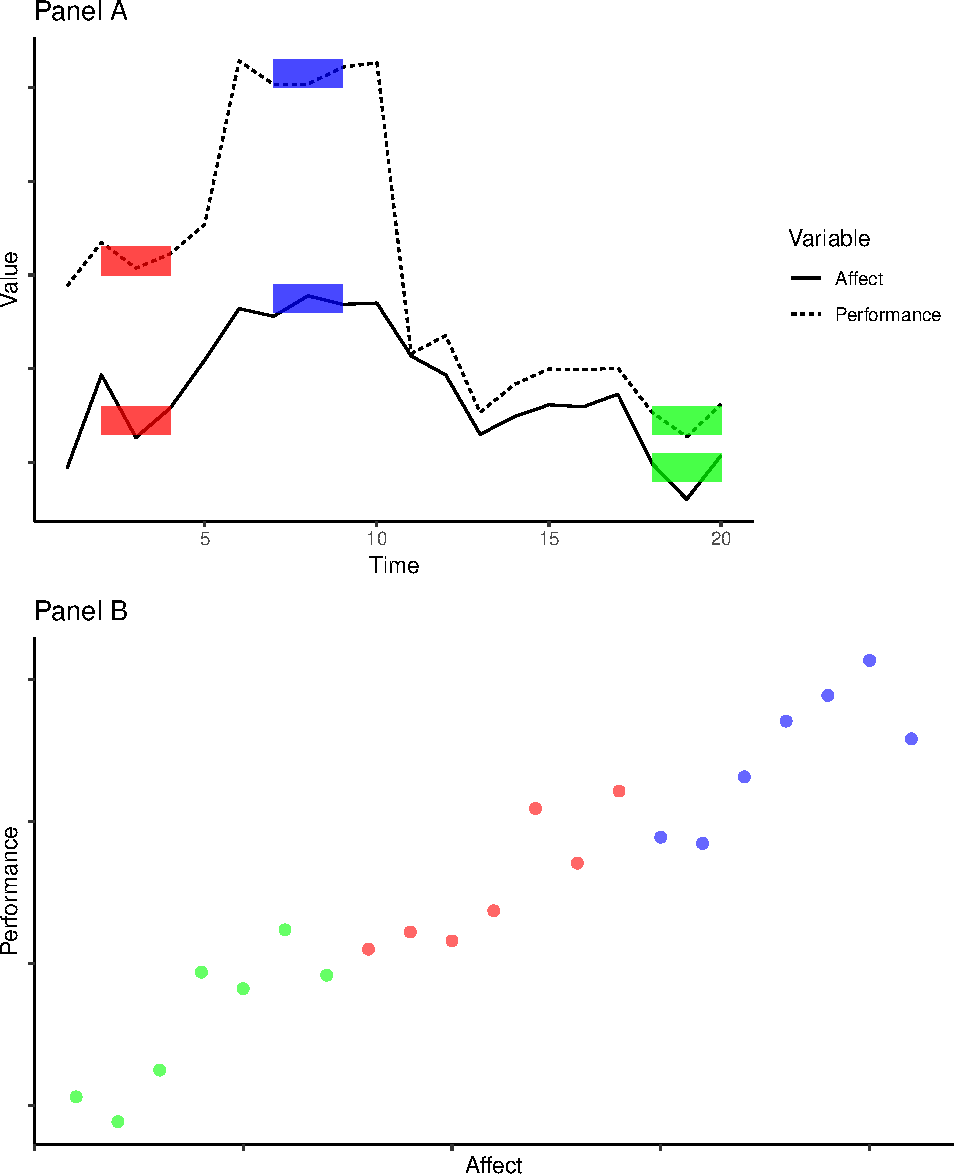
\includegraphics{figures/unnamed-chunk-11-1.pdf}
\caption{\label{fig:unnamed-chunk-11}Between-unit correlation of trend in
affect and performance.\label{trend_correlation}}
\end{figure}

\begin{figure}
\centering
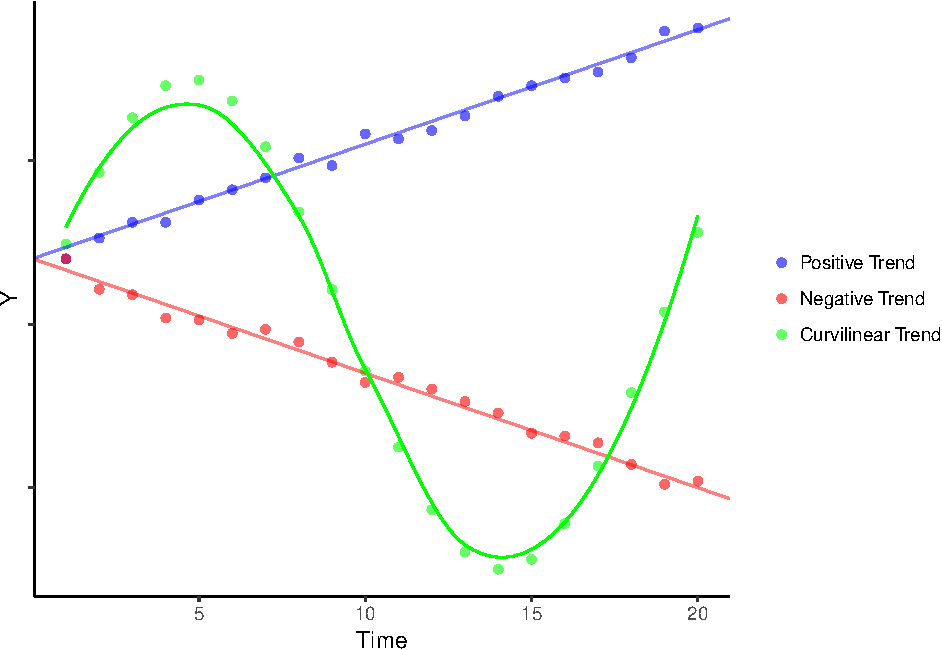
\includegraphics{figures/unnamed-chunk-12-1.pdf}
\caption{\label{fig:unnamed-chunk-12}Job type as a covariate of affect
trend.\label{trend_covariate}}
\end{figure}

\hypertarget{relationships}{%
\section{Relationships}\label{relationships}}

A relationships inference explores between-unit relationships over time.
The second panel of Figure \ref{framework_figure} shows a model
heuristic, where a predictor is concurrently related to a response
variable at each time point and the relationship is typically
constrained to equality or is averaged over time. Essentially, the
inference compiles single-moment between-unit correlations. For example,
we assess the between-unit correlation between, say, OCBs and depletion
at time one, again and times two and three, and then ultimately take the
average of each individual, between-unit correlation.

Questions about static relationships over time take the following forms.
What is the relationship between helping behaviors and incivility? Does
burnout predict turnover intention? Is unethical behavior related to
self-control?

Figure \ref{relation_tvc} shows the inuition of the inference with data.
Panel A plots affect and performance trajectories for three people. The
red circles in Panel A highlight each individual's affect and
performance values at time point six. Given that we have three people at
time point six, we can calculate a correlation between affect and
performance at that moment (granted, it is a small sample). The
calculated coefficient is then graphed in Panel B with another red
circle. At time point six, the between-unit (across people) correlation
among affect and performance is large and positive.

\begin{center}

------------

Insert Figure \ref{relation_tvc} about here

------------

\end{center}

Panel B also shows between-unit correlation coefficients for the rest of
the time points. Often these (between-unit) correlations are either
averaged over time or constrained to be equal. Note that when a
researcher uses a time-varying covariates, hierarchical linear,
random-coefficient, or multi-level model on longitudinal data to explore
concurrent relationships among one or more variables (and they are not
analyzing trend) they are making this inference.

\begin{quote}
\begin{quote}
\textbf{Research Question 1:} What is the average between-unit
relationship of \(x\) and \(y\)? (Typically constrained to be equal over
time or averaged over time).
\end{quote}
\end{quote}

The first relationships inference emphasizes the between-unit expected
average. As with the trend inferences, the next question is to examine
variability in that estimated relationship across the sample. How
consistent across the sample is the relationship between distractions
and fatigue? Is there variability in the relationship between emotions
and volunteering behaviors?

\begin{quote}
\begin{quote}
\textbf{Research Question 2:} What is the variability across units in
the between-unit relationship among \(x\) and \(y\)?
\end{quote}
\end{quote}

\hypertarget{literature-on-statistical-models-for-relationships}{%
\subsection{Literature on Statistical Models for
Relationships}\label{literature-on-statistical-models-for-relationships}}

Time-varying covariates (TVC) analysis is the workhorse behind
relationship inferences. Complete discussions of TVC models are located
in Schonfeld and Rindskopf (2007) and Finch, Bolin, and Kelley (2016)
and two relatively straight-forward empirical examples are in Barnes,
Schaubroeck, Huth, and Ghumman (2011) and Chi, Chang, and Huang (2015).

\begin{figure}
\centering
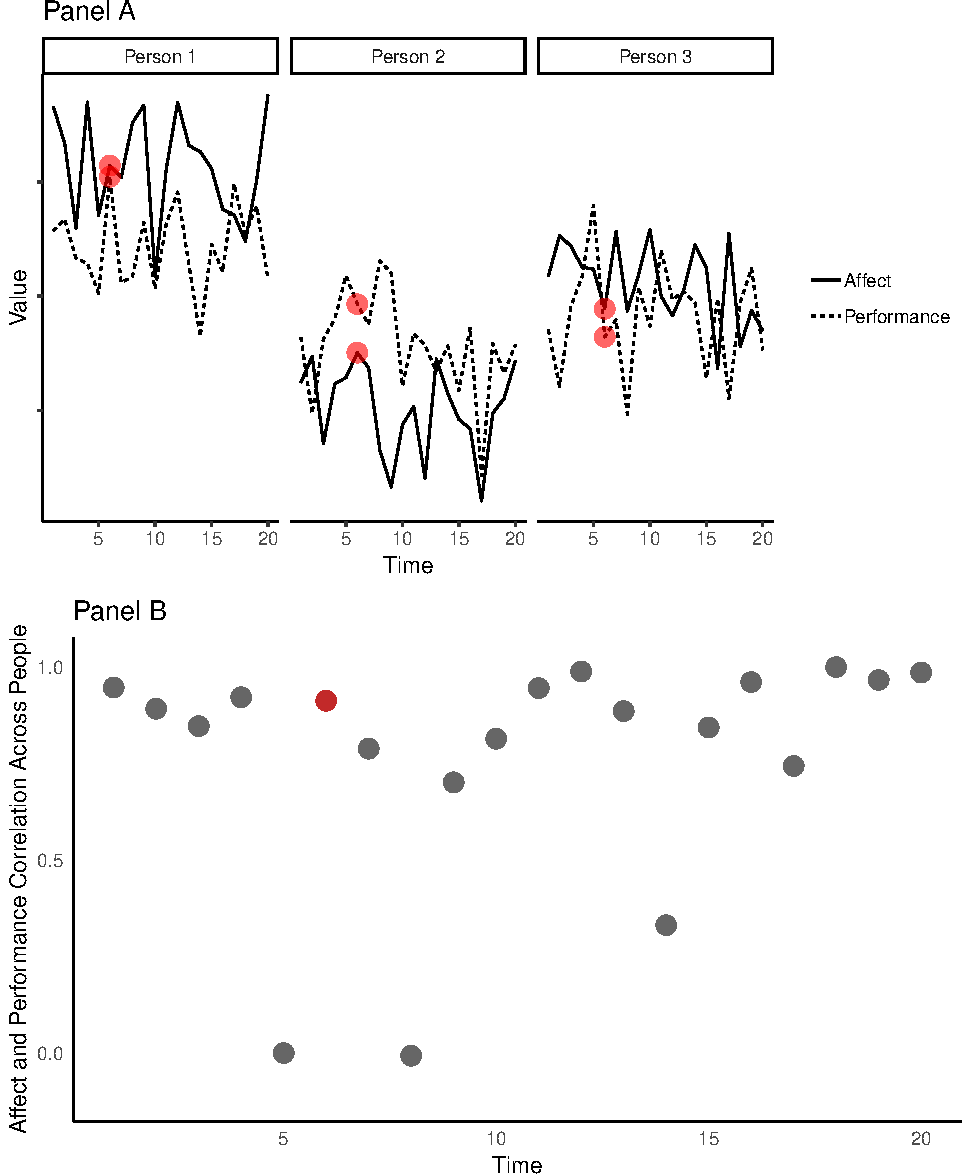
\includegraphics{figures/unnamed-chunk-15-1.pdf}
\caption{\label{fig:unnamed-chunk-15}Relating affect to performance across
units over time. The red circles demonstrate the between unit
correlation at time point six. A typical time-varying covariates model
constrains the correlation to be equivalent across time. Here, the
relationship is unconstrained at each time point.\label{relation_tvc}}
\end{figure}

\hypertarget{dynamics}{%
\section{Dynamics}\label{dynamics}}

The word \enquote{dynamics} takes on a variety of meanings throughout
our literature. Informally, it is used to mean \enquote{change,}
\enquote{fluctuating,} \enquote{longitudinal,} or \enquote{over time}
(among others), but the fundemantal concept to identify with dynamics is
that the past constrains what happens next, variables have memory as
they move through time. For example, Monge (1990) notes that in dynamic
analysis, \enquote{it is essential to know how variables depend upon
their own past history} (p.~409), Vancouver, Wang, and Li (2018) state
that dynamic variables \enquote{behave as if they have memory; that is,
their value at any one time depends somewhat on their previous value}
(p.~604), and Wang, Zhou, and Zhang (2016) define a dynamic model as a
\enquote{representation of a system that evolves over time. In
particular it describes how the system evolves from a given state at
time \emph{t} to another state at time \emph{t + 1} as governed by the
transition rules and potential external inputs} (p.~242). In this
section we discuss a number of inferences couched in the idea that the
past constrains future behavior.

Does performance relate to itself over time? Do current helping
behaviors depend on prior helping behaviors? Does unit climate
demonstrate self-similarity across time? Does income now predict income
in the future? These are questions about the relationship of a single
variable with itself over time -- does it predict itself at each
subsequent moment? Is it constrained by where it was in the past?

Panel A of Figure \ref{dynamics_figure} shows the concept with a
box-and-arrow model heuristic. \(y\) predicts itself across every moment
-- it has self-similarity and its value now is constrained by where it
was a moment ago. In our diagram, we show that \(y\) at time \(t\) is
related to \(y\) at time \(t + 1\). In other words, we posit that \(y\)
shows a lag-one relationship, where \(y\) is related to its future value
one time-step away. Researchers are of course free to suggest any lag
amount that they believe captures the actual relationship. Note that the
statistical term to capture self-similarity or memory is called
autoregression.

\begin{quote}
\begin{quote}
\textbf{Research Question 1:} On average across units, what is the
relationship of \(y\) to itself over time? (Autoregression)
\end{quote}
\end{quote}

\begin{center}

------------

Insert Figure \ref{dynamics_figure} about here

------------

\end{center}

As before, after exploring the expected average we turn to variability.
How consistent are the self-similarity relationships? Are there
between-unit differences in autoregression in, for example, employee
voice? Do we expect a large variance in the autoregression of helping
behaviors?

\begin{quote}
\begin{quote}
\textbf{Research Question 2:} What is the variability across units in
the expected autoregression of \(y\)?
\end{quote}
\end{quote}

The next inference is about relating a predictor to our response
variable while it still retains memory. Panel B of Figure
\ref{dynamics_figure} shows a box-and-arrow diagram: \(y\) is predicted
by concurrent values of \(x\) but it also retains self-similarity. This
model heuristic is therefore said to partial prior \(y\): it examines
the concurrent relationship between \(x\) and \(y\) while statistically
partialling values of \(y\) at \(t - 1\), or statistically accounting
for \(y\) at the prior moment.

Our literature has converged on calling this kind of relationship
\enquote{change} because it emphasizes the difference between \(y\) now
and where it was in the past (e.g., Lanaj et al., 2016; Rosen et al.,
2016). The association asks how current \(x\) relates to the difference
between \(y\) now and its immediately prior value. How does affect
relate to change in performance? Does depletion covary with change in
OCBs? Note that change can be construed from any prior time point
(baseline, \(t-1\), \(t-3\)); our literature commonly emphasizes lag-one
change.

\begin{quote}
\begin{quote}
\textbf{Research Question 3:} On average across units, what is the
relationship betweeen concurrent \(x\) and change in \(y\)?
\end{quote}
\end{quote}

The analyst is also free to assess variability in the expected change
relationship.

\begin{quote}
\begin{quote}
\textbf{Research Question 4:} What is the variability across units in
the expected change relationship between concurrent \(x\) and \(y\)?
\end{quote}
\end{quote}

Change relationships do not have to be concurrent. Panel C of Figure
\ref{dynamics_figure} shows concurrent relationships as we saw above but
it also includes lags from the predictor to the outcome. \(y\) retains
memory, but it is predicted by both concurrent and prior values of
\(x\). Typically, we call these cross-lag relationships.

Questions about lag-one change relationships take the following forms.
Does affect predict subsequent performance change? Do prior
counterproductive work behaviors relate to current incivility change?
Does metacognition predict subsequent exploratory behavior change? Of
course, researchers can also explore longer lags by relating predictors
to more distal outcomes.

\begin{quote}
\begin{quote}
\textbf{Research Question 5:} On average across units, what is the
cross-lag relationship between \(x\) and change in \(y\) at a different
point in time?
\end{quote}
\end{quote}

Again, typically researchers explore variability after assessing the
average estimate.

\begin{quote}
\begin{quote}
\textbf{Research Question 6:} What is the variability over units in the
expected cross-lag relationship of change?
\end{quote}
\end{quote}

\hypertarget{extensions}{%
\subsection{Extensions}\label{extensions}}

We described a simple set of inferences above, but the ideas generalize
to more complex dynamics as well. Often researchers are interested in
reciprocal relationships, where \(x\) influences subsequent \(y\), which
then goes back to influence \(x\) at the next time point. Said formally,
\(x_t\) influences \(y_{t+1}\), which then influences \(x_{t+2}\). Said
informally, current performance influences subsequent self-efficacy,
which then influences performance on the next trial. These inferences
are no different than what we saw above -- they are cross-lag
predictions -- all we did was add more of them. Panel D of Figure
\ref{dynamics_figure} shows reciprocal dynamics, in which both \(x\) and
\(y\) show self-similarity and cross-lag relationships with one another.

Researchers typically posit a sequence of single cross-lag predictions
when they are interested in reciprocal dynamics. For example, Hardy III,
Day, and Steele (2018) explored reciprocal relationships among
performance and motivation (self-efficacy, metacognition, and
exploratory behavior). Their hypotheses include, (1) prior self-efficacy
negatively relates to subsequent exploratory behavior and (2) prior
exploratory behavior positively relates to subsequent self-efficacy
(among others). These single inferences are used in aggregate to make
conclusions about reciprocal influence.

The dynamic inferences shown here also generalize to systems of
variables where a researcher posits self-similarity and cross-lag
predictions across many variables. There could be reciprocal dynamics
between a set of variables like performance, self-efficacy, and affect,
or a sequence of influence between dyadic exchanges, performance, and
team perceptions: perhaps initial dyadic exchanges influence subsequent
team perceptions, which later influence performance. Following the
performance change, the structure of the task updates and this initiates
new dyadic exchanges. Once a researcher grasps the foundational ideas
presented here he or she is free to explore any number of complex
relationships.

\hypertarget{literature-on-statistical-models-for-dynamics}{%
\subsection{Literature on Statistical Models for
Dynamics}\label{literature-on-statistical-models-for-dynamics}}

Wang et al. (2016) review a variety of dynamic models and, although
their paper does not provide readers with specific code, it is an
excellent resource to become familiar with potential dynamic models. Xu,
DeShon, and Dishop (in press) describe why multi-level models are
innapropriate for inferences about dynamics and instead recommend a
general panel model described in Bollen and Brand (2010). Other
statistical models that are appropriate for dynamic inferences are
discussed in Voelkle and Oud (2015), Molenaar (1985); Molenaar and
Nesselroade (2012), Molenaar (2010), McArdle (2009), and Eschleman and
LaHuis (2014).

\begin{figure}

{\centering 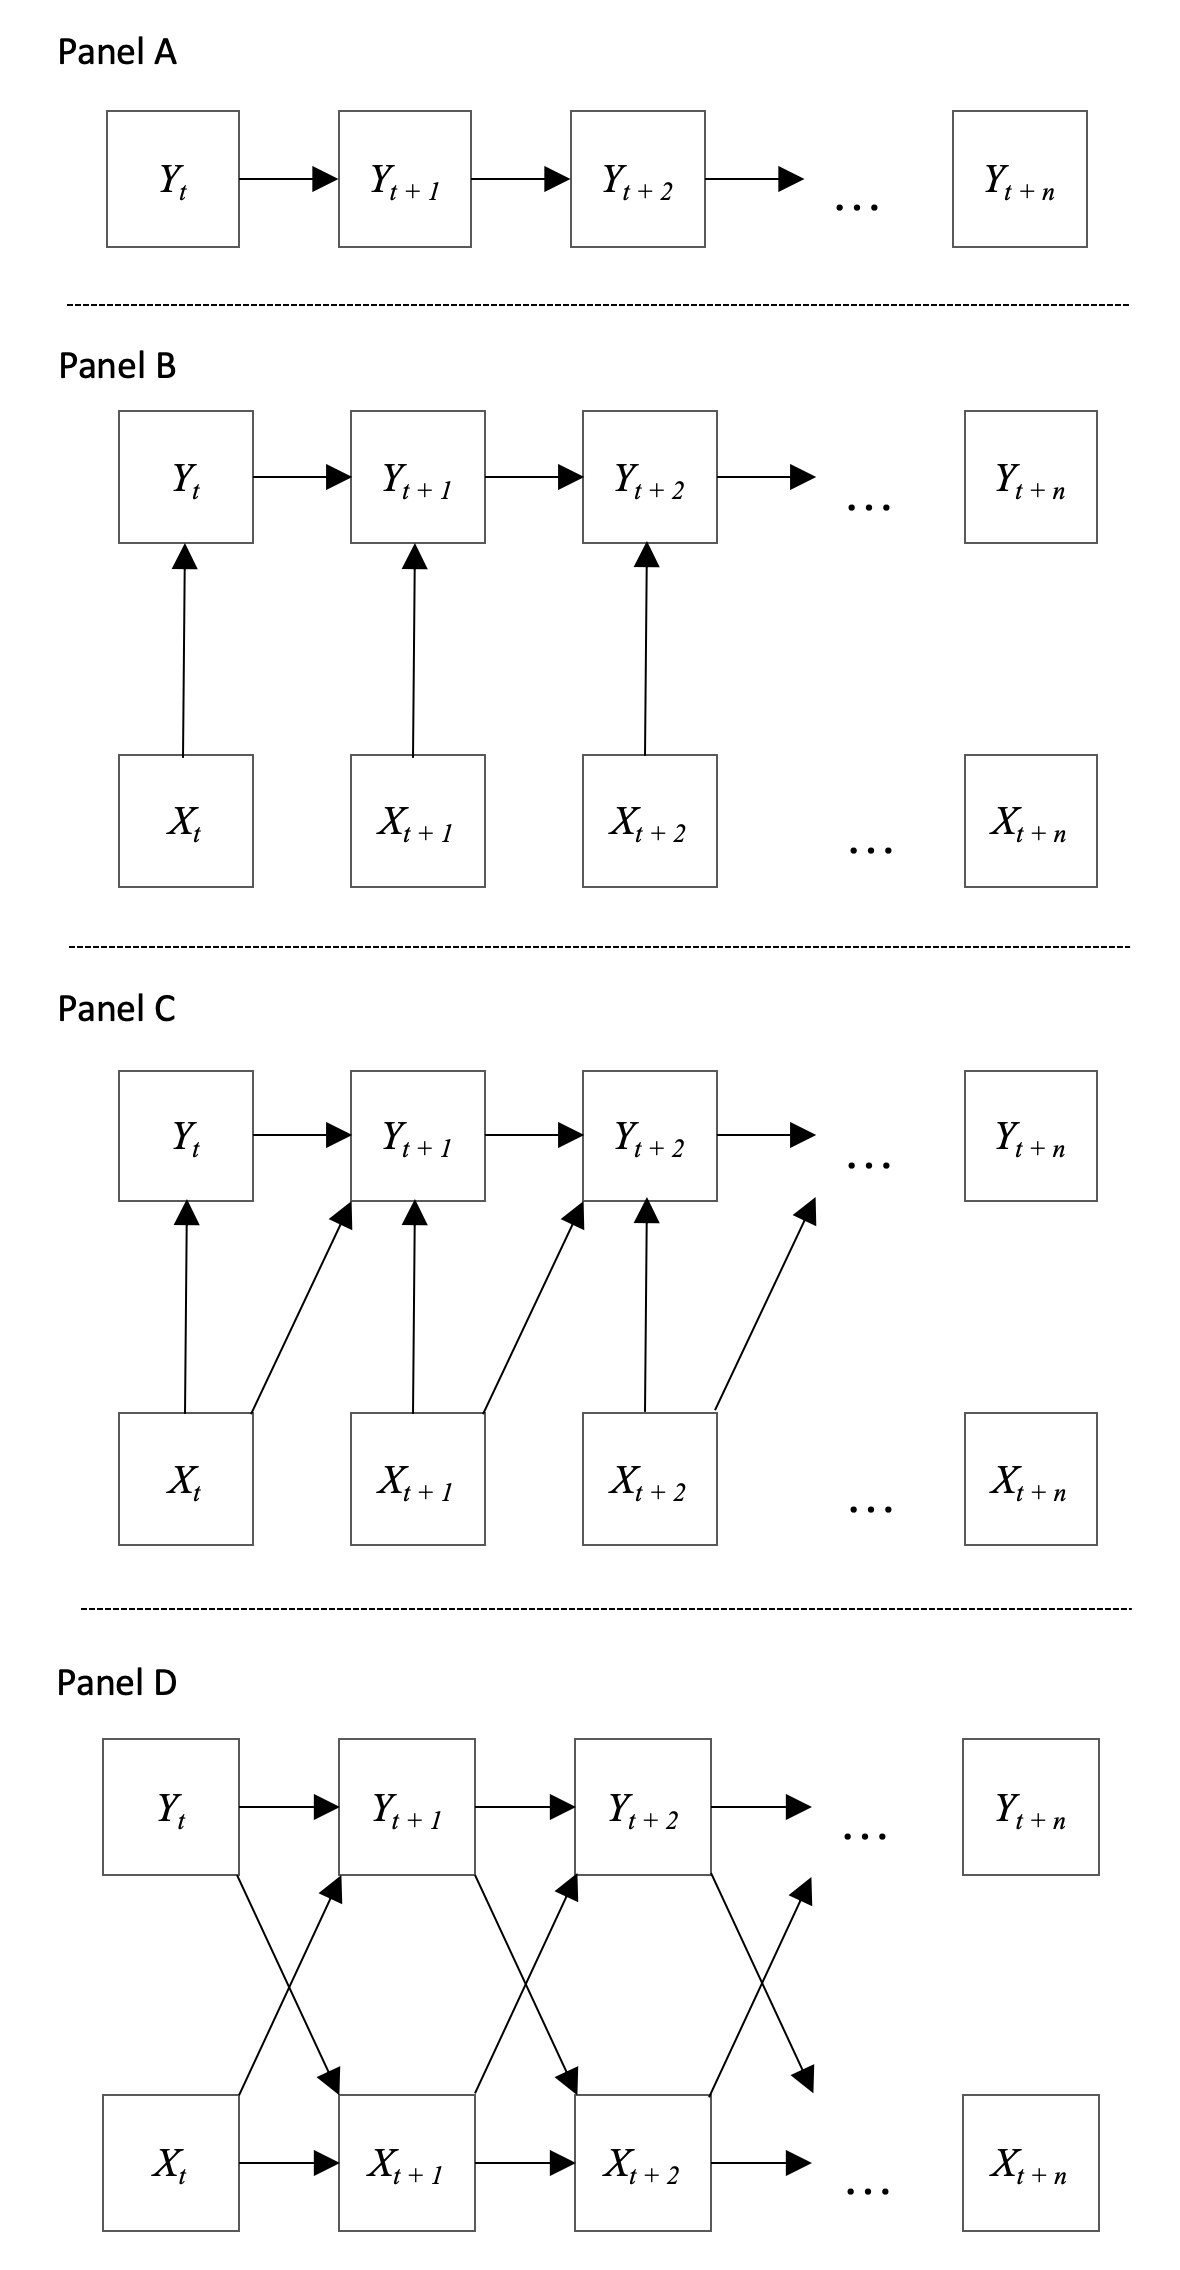
\includegraphics[width=3.93in]{figures/dynamics/dall} 

}

\caption{Univariate and bivariate dynamics adapted from DeShon (2012). Panel A shows self-similarity or autoregression in $Y$ across time. Panel B shows concurrent $X$ predicting change in $Y$. Panel C shows lagged change relationships. Panel D shows reciprocal dynamics between $X$ and $Y$.\label{dynamics_figure}}\label{fig:unnamed-chunk-17}
\end{figure}

\hypertarget{discussion}{%
\section{Discussion}\label{discussion}}

There are many different patterns to explore with longitudinal data
structures. This manuscript, by unpacking between-unit patterns, mirrors
the common questions and inferences currently emphasized by
organizational scientists. What is the between-unit relationship among a
set of constructs (averaged over time)? What is the between-unit
expected trend? Are there between-unit differences in trend (also
phrased as, \enquote{between-unit differences in within-unit change})?
We organized these questions and inferences into a fundamental set,
discussed what they mean, and consolidated disparate literature so that
researchers have a single source to better understand how to think about
over time patterns. Ultimately, researchers should now be able to
understand the spectrum of between-unit inferences that they can explore
with rich, longitudinal data.

Between-unit questions are common and useful and they are the sibling to
an alternative lens to asking questions and making inferences with
repeated measures: within-units. Within-unit inferences emphasize
fluctuations over time rather than across units. For example, Beal
(2015) notes that many of the psychological phenomenon in which we are
interested are \enquote{sequences of events and event reactions that
happen within each person's stream of experience} (p.~5). This is a
within-unit statement: it emphasizes how a construct moves through time
within a single individual. Organizational scientists have become
increasingly interested in within-unit perspectives over the past
decade. Dalal, Bhave, and Fiset (2014) review theory and research on
within-person job performance, Grandey and Gabriel (2015) review
emotional labor and differentiate a variety of within-person
perspectives, Park, Spitzmuller, and DeShon (2013) present a team
motivation model describing within-individual resource allocation and
within-team feedback, Vancouver, Weinhardt, and Schmidt (2010) present a
within-person model of multiple-goal pursuit, Barnes (2012) describes
recent within-person approaches to sleep and organizational behavior,
and Methot, Lepak, Shipp, and Boswell (2017) present a within-person
perspective of organizational citizenship behaviors. There are many
within-person inferences accumulating in our literature, but they are
occasionally accompanied by between-person models or are dispersed and
unconnected among different content areas. An immediate next step for
future research is to create a framework for the fundamental within-unit
inferences.

Our focus was on between-unit patterns because these inferences are the
backbone of longitudinal modeling in organizational science. Moreover,
there can be a tendency for researchers to believe that they are making
within-unit inferences simply because they collect longitudinal data,
our goal was to build consensus and clarity on the fundamental
between-unit ideas in longitudinal data structures. We close the paper
by broadening our view slightly, we discuss two complexities that merit
attention when researchers apply -- irrespective of the inferential lens
that they take -- statistical models to longitudinal data.

When researchers explore patterns in longitudinal data, regardless of
whether they emphasize between or within-unit inferences, there are
additional statistical complexities to consider that influence the
veracity of a researcher's conclusions. For example, consider a
researcher interested in inference one from the \enquote{relationships}
section of this paper. To explore it, she collects data on 400 subjects
across eight time points, applies a recommended statistical model, and
then evaluates the results and makes an inference about the underlying
process. Although she aligned her question with an appropriate
statistical model, there is an issue related to her data that she did
not assess. The longitudinal data that she collected may not contain the
statistical characteristics that merit her inference. She can ask
questions about its patterns, apply a statistical model to it and make
statements that are appropriate \emph{given only the statistical model
that she applied}, but we do not know if her inference is appropriate
\emph{given the statistical characteristics of the data that she applied
her model to}. Do the data merit her inference in the first place?

The statistical complexities that we discuss below include stationarity
and ergodicity. Stationarity and ergodicity are statistical
characteristics that can be assessed with longitudinal data, and we
discuss both below in the context of advocating for greater \(T\), for
researchers to collect more observations over time because statistical
models alone do not reveal stationarity or ergodicity if the analyst is
not meticulously looking for them. They require tests of their own and
the tests are facilitated by data structures with more time points.

Processes give rise to observed data and those observed data are
characterized by distributions and their moments. Stationarity is about
whether or not the statistical characteristics of a process remain
stable over time. When they do, the analyst has permission to use a
variety of regression-based techniques like those described in this
paper without additional concerns of faulty inferences. When
trajectories are non-stationary, however, then the inferences drawn from
regression-based techniques are often misguided (Granger \& Newbold,
1974). Full explanations of stationarity are in Kuljanin et al. (2011b),
Braun et al. (2013), Jebb, Tay, Wang, and Huang (2015), and Metcalfe and
Cowpertwait (2009), we draw attention to it here to emphasize that
studies with greater \(T\) have the ability to assess stationarity and
understand which statistical models are appropriate. Moreover, finding
evidence of (non)stationary is useful theoretical knowledge and needs to
take the foreground of studies that collect longitudinal data.

Ergodicity is another statistical characteristic of a process and it is
important because it determines whether or not researchers can
generalize inferences of inter-individual variability from tests of
between-unit differences to inferences of within-unit variability. To
see the dilemma, consider the following. First, the standard statistical
models in psychology and management, such as growth curves, multi-level
models, mixture modeling, ANOVA, and factor analysis all focus on
between-unit variation (Molenaar, 2004). Second, researchers using these
techniques run their computations on a sample drawn from a population
and then generalize their results back to the population, so (a) the
results live at the level of the population and (b) researchers assume
that the population (or sub population in mixture modeling) is
homogenous (P. C. Molenaar \& Campbell, 2009). These notions are fine on
their own, but often an additional assumption creeps in that is unlikely
to hold: because resuls live at the level of the population and because
researchers assume that the population is homogenous they often also
assume that the results apply to the individuals making up the
population (P. C. Molenaar, 2008b). In other words, they assume that the
results from a test of between-unit variation hold at the level of
within-individual variation.

When processes are ergodic, this implicit assumption holds: the results
of an analysis of between-unit differences generalize to within-unit
patterns and vice versa (Molenaar, 2007; P. C. Molenaar, 2008a).
Researchers can generalize with ergodic processes, they can use a
multi-level model to assess between-unit patterns and then make
statements about within-person relationships. But this generalization is
rarely appropriate. A Gaussian process is non-ergodic if it is
non-stationarity (e.g., it has time-varying trends) and/or heterogeneous
across subjects (subject-specific dynamics). Stated simply, a Gaussian
process is non-ergodic if it has trend and/or Susie's trajectory is
different from Bob's. If either is violated, which is often the case,
then standard analyses of between-subject differences (growth models,
multi-level or random-coefficient models, mixture models, ANOVA, factor
analysis) cannot be used to make within-person statements. In general
(but not always), within-person inferences need to come from unpooled,
subject-specific time-series data structures (P. C. Molenaar, 2009).

Stationarity and ergodicity are complex ideas that merit future
discussion, the point here is that collecting large samples across many
time points allows researchers to assess stationarity and ergodicity and
explore both between and within-unit inferences. Often, though,
researchers have finite resources that force them to decide whether to
emphasize between or within-unit patterns. Your data collection should
align with the inference that you are interested in. If you care about
between-unit patterns (as shown in this paper), focus on \(N\) --
collect data on many participants. If you care about within-unit
patterns, focus on \(T\) -- collect data across many time points. Large
samples across many time points of course gives researchers the ability
to explore both frameworks, but our field will need to recognize that a
small samples (e.g., five or fewer participants) measured across many
time points does allow a researcher to make within-person inferences (by
definition) and is useful. Know your constraints and allocate your
resources accordingly; gather lots of \(N\) when your interest is
between-unit and lots of \(T\) when your interest is within-unit.

\newpage

\hypertarget{references}{%
\section{References}\label{references}}

\setlength{\parindent}{-0.5in}
\setlength{\leftskip}{0.5in}

\hypertarget{refs}{}
\leavevmode\hypertarget{ref-barnes2012working}{}%
Barnes, C. M. (2012). Working in our sleep: Sleep and self-regulation in
organizations. \emph{Organizational Psychology Review}, \emph{2}(3),
234--257.

\leavevmode\hypertarget{ref-barnes_lack_2011}{}%
Barnes, C. M., Schaubroeck, J., Huth, M., \& Ghumman, S. (2011). Lack of
sleep and unethical conduct. \emph{Organizational Behavior and Human
Decision Processes}, \emph{115}(2), 169--180.

\leavevmode\hypertarget{ref-beal_esm_2015}{}%
Beal, D. J. (2015). ESM 2.0: State of the art and future potential of
experience sampling methods in organizational research. \emph{Annu. Rev.
Organ. Psychol. Organ. Behav.}, \emph{2}(1), 383--407.

\leavevmode\hypertarget{ref-bliese_growth_2002}{}%
Bliese, P. D., \& Ployhart, R. E. (2002). Growth modeling using random
coefficient models: Model building, testing, and illustrations.
\emph{Organizational Research Methods}, \emph{5}(4), 362--387.

\leavevmode\hypertarget{ref-bollen_general_2010}{}%
Bollen, K. A., \& Brand, J. E. (2010). A general panel model with random
and fixed effects: A structural equations approach. \emph{Social
Forces}, \emph{89}(1), 1--34.

\leavevmode\hypertarget{ref-braun_spurious_2013}{}%
Braun, M. T., Kuljanin, G., \& DeShon, R. P. (2013). Spurious Results in
the Analysis of Longitudinal Data in Organizational Research.
\emph{Organizational Research Methods}, \emph{16}(2), 302--330.
doi:\href{https://doi.org/10.1177/1094428112469668}{10.1177/1094428112469668}

\leavevmode\hypertarget{ref-chan1998conceptualization}{}%
Chan, D. (1998). The conceptualization and analysis of change over time:
An integrative approach incorporating longitudinal mean and covariance
structures analysis (lmacs) and multiple indicator latent growth
modeling (mlgm). \emph{Organizational Research Methods}, \emph{1}(4),
421--483.

\leavevmode\hypertarget{ref-chi_can_2015}{}%
Chi, N.-W., Chang, H.-T., \& Huang, H.-L. (2015). Can personality traits
and daily positive mood buffer the harmful effects of daily negative
mood on task performance and service sabotage? A self-control
perspective. \emph{Organizational Behavior and Human Decision
Processes}, \emph{131}, 1--15.

\leavevmode\hypertarget{ref-dalal2014within}{}%
Dalal, R. S., Bhave, D. P., \& Fiset, J. (2014). Within-person
variability in job performance: A theoretical review and research
agenda. \emph{Journal of Management}, \emph{40}(5), 1396--1436.

\leavevmode\hypertarget{ref-deshon_multivariate_2012}{}%
DeShon, R. P. (2012). Multivariate dynamics in organizational science.
\emph{The Oxford Handbook of Organizational Psychology}, \emph{1},
117--142.

\leavevmode\hypertarget{ref-dunford_is_2012}{}%
Dunford, B. B., Shipp, A. J., Boss, R. W., Angermeier, I., \& Boss, A.
D. (2012). Is burnout static or dynamic? A career transition perspective
of employee burnout trajectories. \emph{Journal of Applied Psychology},
\emph{97}(3), 637--650.
doi:\href{https://doi.org/http://dx.doi.org.proxy2.cl.msu.edu/10.1037/a0027060}{http://dx.doi.org.proxy2.cl.msu.edu/10.1037/a0027060}

\leavevmode\hypertarget{ref-eschleman_advancing_2014}{}%
Eschleman, K. J., \& LaHuis, D. (2014). Advancing occupational stress
and health research and interventions using latent difference score
modeling. \emph{International Journal of Stress Management},
\emph{21}(1), 112--136.
doi:\href{https://doi.org/10.1037/a0033099}{10.1037/a0033099}

\leavevmode\hypertarget{ref-finch2016multilevel}{}%
Finch, W. H., Bolin, J. E., \& Kelley, K. (2016). \emph{Multilevel
modeling using r}. Crc Press.

\leavevmode\hypertarget{ref-grandey2015emotional}{}%
Grandey, A. A., \& Gabriel, A. S. (2015). Emotional labor at a
crossroads: Where do we go from here?

\leavevmode\hypertarget{ref-granger_spurious_1974}{}%
Granger, C. W., \& Newbold, P. (1974). Spurious regressions in
econometrics. \emph{Journal of Econometrics}, \emph{2}(2), 111--120.

\leavevmode\hypertarget{ref-grimm_growth_2016}{}%
Grimm, K. J., Ram, N., \& Estabrook, R. (2016). \emph{Growth modeling:
Structural equation and multilevel modeling approaches}. Guilford
Publications.

\leavevmode\hypertarget{ref-hardy_interrelationships_2018}{}%
Hardy, J. H., Day, E. A., \& Steele, L. M. (2018). Interrelationships
Among Self-Regulated Learning Processes: Toward a Dynamic Process-Based
Model of Self-Regulated Learning. \emph{Journal of Management},
0149206318780440.
doi:\href{https://doi.org/10.1177/0149206318780440}{10.1177/0149206318780440}

\leavevmode\hypertarget{ref-hardy2018}{}%
Hardy III, J. H., Day, E. A., \& Steele, L. M. (2018).
Interrelationships among self-regulated learning processes: Toward a
dynamic process-based model of self-regulated learning. \emph{Journal of
Management}, 0149206318780440.

\leavevmode\hypertarget{ref-hulsheger_dawn_2016}{}%
Hülsheger, U. R. (2016). From dawn till dusk: Shedding light on the
recovery process by investigating daily change patterns in fatigue.
\emph{Journal of Applied Psychology}, \emph{101}(6), 905--914.
doi:\href{https://doi.org/http://dx.doi.org.proxy2.cl.msu.edu/10.1037/apl0000104}{http://dx.doi.org.proxy2.cl.msu.edu/10.1037/apl0000104}

\leavevmode\hypertarget{ref-ilgen_computational_2000}{}%
Ilgen, D. R., \& Hulin, C. L. (2000). \emph{Computational modeling of
behavior in organizations: The third scientific discipline.} American
Psychological Association.

\leavevmode\hypertarget{ref-jebb2015time}{}%
Jebb, A. T., Tay, L., Wang, W., \& Huang, Q. (2015). Time series
analysis for psychological research: Examining and forecasting change.
\emph{Frontiers in Psychology}, \emph{6}, 727.

\leavevmode\hypertarget{ref-jones_baby_2016}{}%
Jones, K. P., King, E. B., Gilrane, V. L., McCausland, T. C., Cortina,
J. M., \& Grimm, K. J. (2016). The baby bump: Managing a dynamic stigma
over time. \emph{Journal of Management}, \emph{42}(6), 1530--1556.

\leavevmode\hypertarget{ref-judge_what_2014}{}%
Judge, T. A., Simon, L. S., Hurst, C., \& Kelley, K. (2014). What I
experienced yesterday is who I am today: Relationship of work
motivations and behaviors to within-individual variation in the
five-factor model of personality. \emph{Journal of Applied Psychology},
\emph{99}(2), 199.

\leavevmode\hypertarget{ref-kozlowski_advancing_2013}{}%
Kozlowski, S. W., Chao, G. T., Grand, J. A., Braun, M. T., \& Kuljanin,
G. (2013). Advancing multilevel research design: Capturing the dynamics
of emergence. \emph{Organizational Research Methods}, \emph{16}(4),
581--615.

\leavevmode\hypertarget{ref-kozlowski_capturing_2016}{}%
Kozlowski, S. W., Chao, G. T., Grand, J. A., Braun, M. T., \& Kuljanin,
G. (2016). Capturing the multilevel dynamics of emergence: Computational
modeling, simulation, and virtual experimentation. \emph{Organizational
Psychology Review}, \emph{6}(1), 3--33.

\leavevmode\hypertarget{ref-kuljanin2011cautionary}{}%
Kuljanin, G., Braun, M. T., \& DeShon, R. P. (2011a). A cautionary note
on modeling growth trends in longitudinal data. \emph{Psychological
Methods}, \emph{16}(3), 249--264.

\leavevmode\hypertarget{ref-kuljanin_cautionary_2011}{}%
Kuljanin, G., Braun, M. T., \& DeShon, R. P. (2011b). A cautionary note
on modeling growth trends in longitudinal data. \emph{Psychological
Methods}, \emph{16}(3), 249--264.
doi:\href{https://doi.org/http://dx.doi.org.proxy2.cl.msu.edu/10.1037/a0023348}{http://dx.doi.org.proxy2.cl.msu.edu/10.1037/a0023348}

\leavevmode\hypertarget{ref-lanaj_when_2016}{}%
Lanaj, K., Johnson, R. E., \& Wang, M. (2016). When lending a hand
depletes the will: The daily costs and benefits of helping.
\emph{Journal of Applied Psychology; Washington}, \emph{101}(8), 1097.
Retrieved from
\url{http://search.proquest.com/docview/1813203845?pq-origsite=summon}

\leavevmode\hypertarget{ref-mcardle_latent_2009}{}%
McArdle, J. J. (2009). Latent Variable Modeling of Differences and
Changes with Longitudinal Data. \emph{Annual Review of Psychology},
\emph{60}(1), 577--605.
doi:\href{https://doi.org/10.1146/annurev.psych.60.110707.163612}{10.1146/annurev.psych.60.110707.163612}

\leavevmode\hypertarget{ref-mcardle_latent_1987}{}%
McArdle, J. J., \& Epstein, D. (1987). Latent Growth Curves within
Developmental Structural Equation Models. \emph{Child Development},
\emph{58}(1), 110--133.
doi:\href{https://doi.org/10.2307/1130295}{10.2307/1130295}

\leavevmode\hypertarget{ref-metcalfe2009introductory}{}%
Metcalfe, A. V., \& Cowpertwait, P. S. (2009). \emph{Introductory time
series with r}. New York, NY: Chapman; Hall.

\leavevmode\hypertarget{ref-methot2017good}{}%
Methot, J. R., Lepak, D., Shipp, A. J., \& Boswell, W. R. (2017). Good
citizen interrupted: Calibrating a temporal theory of citizenship
behavior. \emph{Academy of Management Review}, \emph{42}(1), 10--31.

\leavevmode\hypertarget{ref-mitchell_building_2001}{}%
Mitchell, T. R., \& James, L. R. (2001). Building better theory: Time
and the specification of when things happen. \emph{Academy of Management
Review}, \emph{26}(4), 530--547.

\leavevmode\hypertarget{ref-molenaar_dynamic_1985}{}%
Molenaar, P. C. (1985). A dynamic factor model for the analysis of
multivariate time series. \emph{Psychometrika}, \emph{50}(2), 181--202.

\leavevmode\hypertarget{ref-molenaar_manifesto_2004}{}%
Molenaar, P. C. (2004). A manifesto on psychology as idiographic
science: Bringing the person back into scientific psychology, this time
forever. \emph{Measurement}, \emph{2}(4), 201--218.

\leavevmode\hypertarget{ref-molenaar2007psychological}{}%
Molenaar, P. C. (2007). Psychological methodology will change profoundly
due to the necessity to focus on intra-individual variation.
\emph{Integrative Psychological and Behavioral Science}, \emph{41}(1),
35--40.

\leavevmode\hypertarget{ref-molenaar2008consequences}{}%
Molenaar, P. C. (2008a). Consequences of the ergodic theorems for
classical test theory, factor analysis, and the analysis of
developmental processes. \emph{Handbook of Cognitive Aging}, 90--104.

\leavevmode\hypertarget{ref-molenaar2008implications}{}%
Molenaar, P. C. (2008b). On the implications of the classical ergodic
theorems: Analysis of developmental processes has to focus on
intra-individual variation. \emph{Developmental Psychobiology: The
Journal of the International Society for Developmental Psychobiology},
\emph{50}(1), 60--69.

\leavevmode\hypertarget{ref-molenaar2009generalization}{}%
Molenaar, P. C. (2009). How generalization works through the single
case: A simple idiographic process analysis of an individual
psychotherapy. In S. Salvatore, J. Valsiner, S. Strout, \& J. Clegg
(Eds.), \emph{YIS: Yearbook of idiographic science} (Vol. 1, pp.
23--38). Rome, Italy: Firera.

\leavevmode\hypertarget{ref-molenaar_testing_2010}{}%
Molenaar, P. C. (2010). Testing all six person-oriented principles in
dynamic factor analysis. \emph{Development and Psychopathology},
\emph{22}(2), 255--259.

\leavevmode\hypertarget{ref-molenaar2009new}{}%
Molenaar, P. C., \& Campbell, C. G. (2009). The new person-specific
paradigm in psychology. \emph{Current Directions in Psychological
Science}, \emph{18}(2), 112--117.

\leavevmode\hypertarget{ref-molenaar_merging_2012}{}%
Molenaar, P. C. M., \& Nesselroade, J. R. (2012). Merging the
Idiographic Filter With Dynamic Factor Analysis to Model Process.
\emph{Applied Developmental Science}, \emph{16}(4), 210--219.
doi:\href{https://doi.org/10.1080/10888691.2012.722884}{10.1080/10888691.2012.722884}

\leavevmode\hypertarget{ref-monge_theoretical_1990}{}%
Monge, P. R. (1990). Theoretical and analytical issues in studying
organizational processes. \emph{Organization Science}, \emph{1}(4),
406--430.

\leavevmode\hypertarget{ref-park2013advancing}{}%
Park, G., Spitzmuller, M., \& DeShon, R. P. (2013). Advancing our
understanding of team motivation: Integrating conceptual approaches and
content areas. \emph{Journal of Management}, \emph{39}(5), 1339--1379.

\leavevmode\hypertarget{ref-pitariu_explaining_2010}{}%
Pitariu, A. H., \& Ployhart, R. E. (2010). Explaining change: Theorizing
and testing dynamic mediated longitudinal relationships. \emph{Journal
of Management}, \emph{36}(2), 405--429.

\leavevmode\hypertarget{ref-ployhart_longitudinal_2010}{}%
Ployhart, R. E., \& Vandenberg, R. J. (2010). Longitudinal research: The
theory, design, and analysis of change. \emph{Journal of Management},
\emph{36}(1), 94--120.

\leavevmode\hypertarget{ref-rosen_who_2016}{}%
Rosen, C. C., Koopman, J., Gabriel, A. S., \& Johnson, R. E. (2016). Who
strikes back? A daily investigation of when and why incivility begets
incivility. \emph{Journal of Applied Psychology}, \emph{101}(11), 1620.

\leavevmode\hypertarget{ref-schonfeld2007hierarchical}{}%
Schonfeld, I. S., \& Rindskopf, D. (2007). Hierarchical linear modeling
in organizational research: Longitudinal data outside the context of
growth modeling. \emph{Organizational Research Methods}, \emph{10}(3),
417--429.

\leavevmode\hypertarget{ref-scott_multilevel_2011}{}%
Scott, B. A., \& Barnes, C. M. (2011). A multilevel field investigation
of emotional labor, affect, work withdrawal, and gender. \emph{Academy
of Management Journal}, \emph{54}(1), 116--136.

\leavevmode\hypertarget{ref-singer_applied_2003}{}%
Singer, J. D., Willett, J. B., \& Willett, J. B. (2003). \emph{Applied
longitudinal data analysis: Modeling change and event occurrence}.
Oxford university press.

\leavevmode\hypertarget{ref-vancouver_translating_2018}{}%
Vancouver, J. B., Wang, M., \& Li, X. (2018). Translating Informal
Theories Into Formal Theories: The Case of the Dynamic Computational
Model of the Integrated Model of Work Motivation. \emph{Organizational
Research Methods}, 109442811878030.
doi:\href{https://doi.org/10.1177/1094428118780308}{10.1177/1094428118780308}

\leavevmode\hypertarget{ref-vancouver2010formal}{}%
Vancouver, J. B., Weinhardt, J. M., \& Schmidt, A. M. (2010). A formal,
computational theory of multiple-goal pursuit: Integrating goal-choice
and goal-striving processes. \emph{Journal of Applied Psychology},
\emph{95}(6), 985.

\leavevmode\hypertarget{ref-voelkle2015relating}{}%
Voelkle, M. C., \& Oud, J. H. (2015). Relating latent change score and
continuous time models. \emph{Structural Equation Modeling: A
Multidisciplinary Journal}, \emph{22}(3), 366--381.

\leavevmode\hypertarget{ref-Wang2016}{}%
Wang, M., Zhou, L., \& Zhang, Z. (2016). Dynamic modeling. \emph{Annual
Review of Organizational Psychology and Organizational Behavior},
\emph{3}(1), 241--266.
doi:\href{https://doi.org/10.1146/annurev-orgpsych-041015-062553}{10.1146/annurev-orgpsych-041015-062553}

\leavevmode\hypertarget{ref-wildman2012trust}{}%
Wildman, J. L., Shuffler, M. L., Lazzara, E. H., Fiore, S. M., Burke, C.
S., Salas, E., \& Garven, S. (2012). Trust development in swift starting
action teams: A multilevel framework. \emph{Group \& Organization
Management}, \emph{37}(2), 137--170.

\leavevmode\hypertarget{ref-xu_deshon_dishop}{}%
Xu, R., DeShon, R. P., \& Dishop, C. R. (n.d.). Challenges and
opportunities in the estimation of dynamic models. \emph{Organizational
Research Methods}.


\end{document}
